\chapter{Ευστάθεια}\label{ch:stab}
Τα συστήματα σχεδιάζονται ώστε να εκτελούν κάποιες εργασίες. Αν ένα σύστημα δεν
είναι ευσταθές τότε το σύστημα μπορεί να χαλάσει, μπορεί να αποτύχει να εκτελέσει
την εργασία ή να εκτελεσθεί μερικώς. Επομένως στην πράξη ένα ασταθές σύστημα δεν
είναι αξιοποιήσιμο και η ευστάθεια είναι μία βασική προδιαγραφή που πρέπει κάθε
σύστημα να ικανοποιεί.

Η έννοια της ευστάθειας που συναντάται συνήθως στη μελέτη των δυναμικών
συστημάτων και της θεωρίας ελέγχου είναι η ευστάθεια κατά \tl{Lyapunov} και αυτή
θα παρουσιάσουμε. Οι μαθηματικοί ορισμοί που θα ακολουθήσουν είναι από το
βιβλίο~\cite{hirsch1974differential}.

Θεωρούμε ότι η δυναμική συμπεριφορά ενός συστήματος μοντελοποιείται μαθηματικά
από τις λύσεις του δυναμικού συστήματος
\begin{equation}\label{eq:stab_ode}
    \dot{x} = f(x), \quad f:U \to \mathbb{R}^n.
\end{equation}
Ενδιαφερόμαστε για την μακροπρόθεσμη συμπεριφορά των τροχιών της παραπάνω.
Ιδιαίτερο ενδιαφέρον παρουσιάζουν τα σημεία ισορροπίας. Τέτοια σημεία
\( \bar{x} \in U \) είναι αυτά που δεν αλλάζουν με το χρόνο. Μαθηματικά, αυτό
σημαίνει ότι η σταθερή απεικόνιση \( t \to \bar{x} \) είναι λύση του δυναμικού
συστήματος, ή ισοδύναμα, \( f(\bar{x}) = 0 \). Έτσι ορίζουμε \emph{σημείο
ισορροπίας} της~\eqref{eq:stab_ode} το σημείο \( \bar{x} \in U \) τέτοιο ώστε \(
f(\bar{x}) = 0 \).

\section{Ευστάθεια κατά \tl{Lyapunov}}
Θεωρούμε ότι ένα σημείο ισορροπίας είναι ευσταθές αν λύσεις που ξεκινούν
\enquote*{κοντά σε αυτό}, παραμένουν \enquote*{κοντά σε αυτό} για κάθε μελλοντικό χρόνο.
Ο μαθηματικοί ορισμοί της ευστάθειας κατά \tl{Lyapunov} διατυπώνονται παρακάτω.

\begin{definition} [Ευστάθεια κατά \tl{Lyapunov}, των \tl{Hirsch} και
    \tl{Smale}~\cite{hirsch1974differential}]
    Έστω \( \bar{x} \in W \) σημείο ισορροπίας της διαφορικής εξίσωσης
    \[
        \dot{x} = f(x),
    \]
    όπου \( f: W \to E \) είναι \( C^1 \) συνάρτηση από το ανοιχτό σύνολο \( W
    \) του διανυσματικού χώρου \( E \) στο \( E \). Τότε το \( \bar{x} \) είναι
    \emph{ευσταθές} σημείο ισορροπίας αν για κάθε γειτονιά \( U \) του \( \bar{x} \)
    του \( W \) υπάρχει γειτονιά \( U_1 \) του \( \bar{x} \) στο \( U \) τέτοια
    ώστε κάθε λύση \( x(t) \) με \( x(0) \) στο \( U_1 \) να ορίζεται στο \( U
    \) για κάθε \( t > 0 \).
\end{definition}
\begin{figure}[h!]
    \centering
    \includegraphics[width=0.3\textwidth]{figures/stab_stable.eps}
    \caption{Ευσταθές σημείο ισορροπίας}
    \label{fig:stab_stable}
\end{figure}
\begin{definition} [Ασυμπτωτική ευστάθεια κατά \tl{Lyapunov}, των \tl{Hirsch} και
    \tl{Smale}~\cite{hirsch1974differential}]
    Αν το \( U_1 \) μπορεί να επιλεγεί έτσι ώστε να ισχύουν τα όσα περιγράφηκαν
    στον παραπάνω ορισμό και \( \lim_{t \to \infty} x(t) = \bar{x} \), τότε το \( \bar{x}
    \) είναι \emph{ασυμπτωτικά ευσταθές}.
\end{definition}
\begin{figure}[h!]
    \centering
    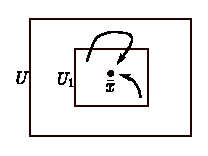
\includegraphics[width=0.3\textwidth]{figures/stab_asymp_stable.eps}
    \caption{Ασυμπτωτικά ευσταθές σημείο ισορροπίας}
    \label{fig:stab_asymp_stable}
\end{figure}
\begin{definition} [Αστάθεια κατά \tl{Lyapunov}, των \tl{Hirsch} και
    \tl{Smale}~\cite{hirsch1974differential}]
    Ένα σημείο ισορροπίας \( \bar{x} \) που δεν είναι ευσταθές είναι
    \emph{ασταθές}. Αυτό σημαίνει ότι υπάρχει γειτονιά \( U \) του \( \bar{x} \)
    τέτοια ώστε για κάθε γειτονιά \( U_1 \) του \( \bar{x} \) στο \( U \),
    υπάρχει τουλάχιστον μία λύση \( x(t) \) που ξεκινάει από το \( x(0) \in U_1 \)
    και δε βρίσκεται στο \( U \).
\end{definition}
\begin{figure}[h!]
    \centering
    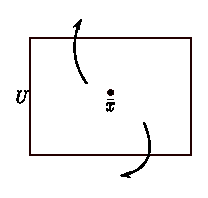
\includegraphics[width=0.3\textwidth]{figures/stab_unstable.eps}
    \caption{Ασταθές σημείο ισορροπίας}
    \label{fig:stab_unstable}
\end{figure}

Πρέπει να σημειωθεί ότι μόνο η σύγκλιση στο σημείο ισορροπίας στον δεύτερο
ορισμό, δεν αρκεί για να χαρακτηριστεί το σημείο ασυμπτωτικά ευσταθές για
γενική συνάρτηση \( f \) της σχέσης~\eqref{eq:stab_ode}. Παρόλο αυτά
αποδεικνύεται ότι αν το υπό μελέτη σύστημα είναι γραμμικό και χρονικά αναλλοίωτο
τότε η έννοια της σύγκλισης συμπίπτει με την έννοια της ασυμπτωτικής ευστάθειας.
Με τους παραπάνω ορισμούς μπορούμε να χαρακτηρίσουμε ένα σημείο ισορροπίας ως
προς την ευστάθεια του μέσω των ιδιοτιμών της γραμμικοποίησης. Παρόλο αυτά με
την τεχνική αυτή, η ευστάθεια δε μπορεί να διαπιστωθεί για κάθε περίπτωση. Ο
Ρώσος μαθηματικός και μηχανικός \tl{Lyapunov} στη διδακτορική του διατριβή μας
έδωσε ένα χρήσιμο κριτήριο περί ευστάθειας. Προτού διατυπώσουμε το θεώρημα θα
δώσουμε κάποιους συμβολισμούς.

Έστω \( V: V \to \mathbb{R} \) διαφορίσιμη συνάρτηση σε μία γειτονιά \( U
\subset W \) του \( \bar{x} \). Συμβολίζουμε με \( \dot{V}: U \to \mathbb{R} \)
τη συνάρτηση που ορίζεται
\[
    \dot{V}(x) = DV(x)(f(x)).
\]
Το δεξί μέλος της παραπάνω είναι απλώς ο τελεστής \( DV(x) \) εφαρμοσμένος στο
διάνυσμα \( f(x) \). Τότε αν \( \phi_t(x) \) είναι η λύση
της~\eqref{eq:stab_ode} που περνάει από το \( x \) όταν \( t = 0 \), προκύπτει
\[
    \dot{V}(x) = \frac{d}{dt}V(\phi_t(x))\big\rvert_{t = 0},
\]
από τον κανόνα της αλυσίδας. Συνεπώς, αν \( \dot{V}(x) \) είναι αρνητικό, τότε η
\( V \) μειώνεται συναρτήσει της λύσης της~\eqref{eq:stab_ode} ως προς το \( x
\). Ο ορισμός του θεωρήματος ευστάθειας του \tl{Lyapunov} διατυπώνεται
παρακάτω.

\begin{theorem} [Άμεση μέθοδος \tl{Lyapunov}, των \tl{Hirsch} και
    \tl{Smale}~\cite{hirsch1974differential}]
    Έστω \( \bar{x} \in W \) σημείο ισορροπίας της~\eqref{eq:stab_ode}. Έστω \(
    V: U \to \mathbb{R} \) συνεχής συνάρτηση ορισμένη σε μία γειτονιά \( U
    \subset W \) του \( x \), διαφορίσιμη στο \( U - \bar{x} \), τέτοια ώστε
    \begin{enumerate} [label = (\enumgreek*)]
        \item \( V(\bar{x}) = 0 \) και \( V(x) > 0 \) αν \( x \neq
            \bar{x} \),
        \item \( \dot{V} \leq 0 \) στο \( U - \bar{x} \).
    \end{enumerate}
    Τότε το \( \bar{x} \) είναι ευσταθές. Επιπλέον, αν ακόμη
    \begin{enumerate} [label = (\enumgreek*),resume]
        \item \( \dot{V} <  0 \) στο \( U - \bar{x} \),
    \end{enumerate}
    τότε το \( \bar{x} \) είναι ασυμπτωτικά ευσταθές.
\end{theorem}

Συνάρτηση \( V \) που ικανοποιεί τα \emph{(α)} και \emph{(β)} ονομάζεται συνάρτηση
\tl{Lyapunov} για το \( \bar{x} \). Αν ακόμη ικανοποιεί για το \emph{(γ)}, τότε
ονομάζεται αυστηρή συνάρτηση \tl{Lyapunov}.

Το πλεονέκτημα του θεωρήματος του \tl{Lyapunov} είναι ότι μπορεί να εφαρμοστεί
χωρίς να λύσουμε τη διαφορική εξίσωση. Από την άλλη, δεν υπάρχει κάποια
συγκεκριμένη μέθοδος για να βρούμε συναρτήσεις \tl{Lyapunov}. Σε περιπτώσεις
μηχανολογικών και ηλεκτρικών συστημάτων, η συνάρτηση της συνολική ενέργεια είναι
καλή υποψήφια συνάρτηση \tl{Lyapunov}. Για περαιτέρω παραπέμπουμε στις
δημοσιεύσεις του \tl{Lyapunov}~\cite{lyapunov1992general} και στα
βιβλία~\cite{hirsch1974differential}.

\section{Ευστάθεια αυτόνομου γραμμικού αναλλοίωτου συστήματος}
Το παραπάνω θεώρημα του \tl{Lyapunov} απλοποιείται σημαντικά στην περίπτωση που
έχουμε γραμμικό και χρονικά αναλλοίωτο σύστημα της μορφής
\begin{equation}\label{eq:stab_auto}
    \dot{x}(t) = Ax(t),\quad x(0) = x_0.
\end{equation}
Γνωρίζουμε ότι το σύστημα είναι ασυμπτωτικά ευσταθές αν όλες οι ιδιοτιμές του
\( A \) έχουν αρνητικό πραγματικό μέρος. Ο πίνακας \( A \) τότε λέγεται
\tl{Hurwitz} πίνακας. Έτσι έχουμε την πρόταση:
\begin{prop} [Πρόταση 2.1 των \tl{Dullerud} και
    \tl{Paganini}~\cite{dullerud2005course}]
    Το αυτόνομο σύστημα~\eqref{eq:stab_auto} είναι εσωτερικά ευσταθές αν και
    μόνο αν ο πίνακας \( A \) είναι \tl{Hurwitz}.
\end{prop}

Το ισοδύναμο θεώρημα του \tl{Lyapunov} για το παραπάνω σύστημα σύμφωνα
με το βιβλίο~\cite{chen1999linear}, είναι το εξής:
\begin{theorem} [Θεώρημα 5.5 του \tl{Chen}~\cite{chen1999linear}]
    Όλες οι ιδιοτιμές του \( A \) έχουν αρνητικό πραγματικό μέρος αν και μόνο αν
    για κάποιον θετικά ορισμένο συμμετρικό πίνακα \( N \), η συνάρτηση
    \tl{Lyapunov}
    \[
        A^{T}M + MA = -N,
    \]
    έχει μοναδική συμμετρική λύση \( M \) και ο \( M \) είναι θετικά ορισμένος.
\end{theorem}
Επίσης, για τον υπολογισμό του πίνακα \( M \) προκύπτει το παρακάτω θεώρημα.
\begin{theorem} [Θεώρημα 5.6 του \tl{Chen}~\cite{chen1999linear}]
    Αν όλες οι ιδιοτιμές του \( A \) έχουν αρνητικό πραγματικό μέρος,
    τότε η συνάρτηση \tl{Lyapunov}
    \[
        A^{T}M + MA = -N,
    \]
    έχει μοναδική λύση για κάθε \( N \), και η λύση μπορεί να εκφραστεί ως
    \[
        M = \int_0^{\infty}e^{A^{T}t}Ne^{At} \, dt.
    \]
\end{theorem}

Όσα αναφέραμε παραπάνω αφορούν αυτόνομα συστήματα της
μορφής~\eqref{eq:stab_ode}. Στα συστήματα ελέγχου συνήθως, η είσοδος έχει
μορφή ανάδρασης της κατάστασης, δηλαδή συνάρτηση του \( x \). Έτσι με τους παραπάνω
ορισμούς και θεωρήματα έχοντας την είσοδο ως \( u(x) \) μπορούμε να αποφανθούμε
για την ευστάθεια του συστήματος.

\section{Ευστάθεια γραμμικού αναλλοίωτου συστήματος ελέγχου}
Δοθέντος συστήματος της μορφής
\begin{equation}\label{eq:stab_control}
    \dot{x}(t) = Ax(t) + Bu(t), \quad x(0) = x_0,
\end{equation}
με \( x(t) \in \mathbb{R}^n, u(t) \in \mathbb{R}^m \),
τότε ονομάζουμε τον πίνακα
\[
    \begin{bmatrix}
        B & AB & A^2B & \dots & A^{n - 1}B
    \end{bmatrix}
\]
πίνακα ελεγξιμότητας. Όταν ο πίνακας έχει πλήρη βαθμό \( n \), τότε λέμε ότι το
ζεύγος \( (A, B) \) είναι ελέγξιμο, ή αντίστοιχα ότι το σύστημα είναι ελέγξιμο.
Αν βρούμε ένα νόμο ανάδρασης της μορφής \( u(t) = Fx(t) \) με \( F \) σταθερό
πίνακα στο \( \mathbb{R}^{m \times n} \), τότε η παραπάνω γίνεται
\[
    \dot{x}(t) = (A + BF)x(t), \quad x(0) = x_0.
\]
Τότε έχουμε το παρακάτω θεώρημα.
\begin{theorem} [Θεώρημα 2.19 των \tl{Dullerud} και
    \tl{Paganini}~\cite{dullerud2005course}]
    Οι ιδιοτιμές του \( A + BF \) είναι ελεύθερα επιλέξιμες, επιλέγοντας τον
    πίνακα \( F \in \mathbb{R}^{m \times n} \), αν και μόνο αν το ζεύγος \( (A,
    B) \) είναι ελέγξιμο.
\end{theorem}
Στην πράξη, πολύ συχνά μελετούμε γραμμικά αναλλοίωτα συστήματα της
μορφής~\eqref{eq:stab_control}, όπου η ανάδραση είναι γραμμική συνάρτηση
των καταστάσεων. Στις περιπτώσεις αυτές έχουμε μία ικανή και
αναγκαία συνθήκη ώστε να μετατρέψουμε το πιθανόν ασταθές αυτόνομο σύστημα σε
ευσταθές ή να επιλέξουμε σύμφωνα με κάποια κριτήρια τις ιδιοτιμές του κλειστού
συστήματος με κατάλληλη επιλογή του πίνακα \( F \).

Πολλές φορές όταν η είσοδος είναι μη μηδενική συναντούμε συχνά δύο τύπους
ευστάθειας. Σύμφωνα με το βιβλίο~\cite{brogan1991modern} οι ορισμοί είναι:

\begin{definition} [Ορισμός 10.3 του \tl{Brogan}~\cite{brogan1991modern}]
    Αν υπάρχει ένας σταθερός, πεπερασμένος και σταθερός \( K \) τέτοιος ώστε
    \( \|u\| \leq K \) για κάθε χρόνο \( t \), τότε η είσοδος λέμε ότι είναι φραγμένη.
    Αν για κάθε φραγμένη είσοδο, και για οποιαδήποτε αρχική συνθήκη
    \( x(t_0) \), υπάρχει θετικό βαθμωτό \( \delta(K, t_0, x(t_0)) \) τέτοιο
    ώστε η επακόλουθη κατάσταση να ικανοποιεί \( \|x\| \leq \delta \), τότε το
    σύστημα λέμε ότι είναι φραγμένης εισόδου, φραγμένης κατάστασης ευσταθές, γνωστό και
    ως \tl{BIBS}.
\end{definition}

Οι παραπάνω ορισμοί της ευστάθειας αντιμετωπίζουν τη συμπεριφορά του διανύσματος
κατάστασης ως προς ένα σημείο ισορροπίας. Πολλές φορές, το βασικό ενδιαφέρον
είναι η συμπεριφορά της εξόδου του συστήματος. Έτσι έχουμε τον ακόλουθο ορισμό
περί ευστάθειας.

\begin{definition} [Ορισμός 10.4 του \tl{Brogan}~\cite{brogan1991modern}]
    Έστω \( u \) φραγμένη είσοδος με \( K_m \) το ελάχιστο πάνω φράγμα. Αν
    υπάρχει βαθμωτό \( a \) τέτοιο ώστε για κάθε χρόνο \( t \), η έξοδος
    ικανοποιεί \( \|y\| \leq aK_m \), τότε το σύστημα λέμε ότι είναι φραγμένης
    εισόδου, φραγμένης εξόδου ευσταθές, γνωστό και ως \tl{BIBO}.
\end{definition}

Η έννοια της ευστάθειας εισόδου, εξόδου γενικεύονται και ορίζεται μέσω των χώρων
\( L_p \). Για περαιτέρω παραπέμπουμε στο βιβλίο~\cite{vidyasagar2002nonlinear}.
